\section{Introduction}

In a true many-body electronic wave function, the motions of electrons are correlated across the entire range of interelectronic distances.
The (in principle exact) Kohn--Sham density functional theory (KS-DFT)~\cite{KohnPR65} captures all the correlations in the form of the exchange--correlation (XC) energy.
Many approximate functionals are able to efficiently estimate most of the XC energy, which established KS-DFT as a basic tool in computational chemistry and condensed-matter physics.
But the standard approximations are semilocal in space, resulting in XC energy that decays exponentially with distance---as if the electrons were essentially uncorrelated at long range (except for the special case of slowly-varying electron density).
This leads to severe underestimation of van der Waals (vdW) dispersion interactions, which are mostly caused by long-range electron correlation.
As these interactions strongly contribute to properties of nearly all biological and modern synthetic materials, many models were developed that account specifically for the long-range correlation~\cite{DionPRL04,VydrovJCP10a,JohnsonJCP06,TkatchenkoPRL09,GrimmeJCP10,AmbrosettiJCP14} to augment the semilocal (or hybrid) density-functional calculations.
The range separation of electron correlation into short-range and long-range models can be in principle done formally~\cite{HermannCR17}, but insufficient knowledge about the ranges of different semilocal functionals prevents this in practice.
The vdW methods range from interatomic pairwise sums, to spatial double-integral functionals, to Hamiltonian many-body models, but in all these cases the issue of range separation can be reduced to empirical damping mechanisms that couple the semilocal and nonlocal contributions to the electron correlation.

Fitting empirical damping functions to benchmark binding energies has three associated issues, all of which decrease the transferability and hence generality of the resulting DFT+vdW methods.
First, the asymptotic binding energies predicted by the approximate vdW models may have both systematic and unsystematic errors, which can be ``fixed'' by the fitting only for a fairly small class of systems.
Second, the effective range of the semilocal functionals may systematically depend on the system type.
The fitted damping function would then strongly depend on the selection of the training set.
Third, this approach assumes that the only error in the KS-DFT energies is the missing long-range correlation, where in fact other noncovalent interactions may also be estimated incorrectly by the approximate semilocal functionals.
The fitting then effectively corrects for these errors, but such compensation is nontransferable to systems besides the training set.
These issues could be largely solved if the effective range of the semilocal functionals was well-defined, which would restrict the form of the damping functions, limiting the chance of spurious error overcorrection.
Understanding the effective range of current semilocal functionals is then a first step toward a more systematic range separation in the DFT+vdW methods.

Traditionally, the differences between XC functionals in their contribution to the binding in vdW systems have been formulated in terms of strength rather than range.
Whereas the strength is attested simply by the magnitude of binding energies at equilibrium geometries, the range is more subtle and decides about the rate of decay of the binding when the interacting objects are moved apart, as well as about the scaling of the binding energies with system size.
Besides numerical results, the strength of the vdW binding by different XC functionals has been often analyzed analytically via the so-called enhancement factor, $F_\text{XC}$.
But this approach is not well-transferable to the analysis of the effective range
Instead, we chose to study the range by careful analysis of the binding energies across a range of intermolecular distances and system sizes.
To this end, we employ several vdW benchmark data sets from small noncovalently bonded organic dimers, to molecular crystals, to supramolecular complexes, as well as a series of graphene-flake dimers of increasing size.
With the use of the range-separation parameters in vdW methods, we are then able to deduce information about the effective ranges of XC functionals that would not be possible from the analysis of $F_\text{XC}$.

\begin{figure}[t!]
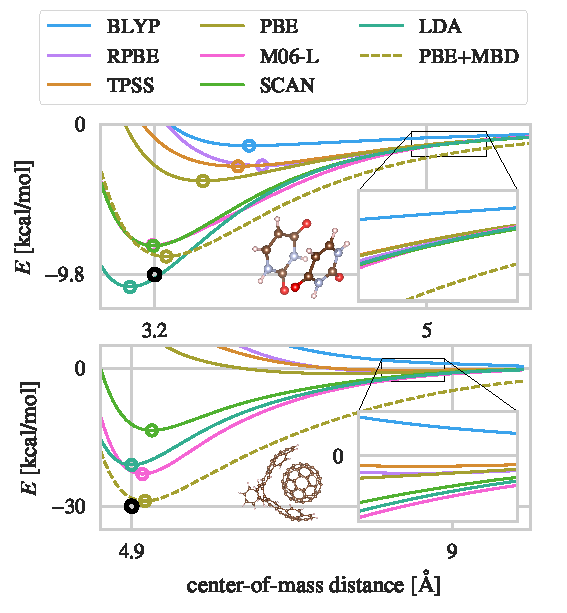
\includegraphics[center]{media/range-curves}
\caption{\textbf{Range of functionals.}
Binding energy curves of a stacked uracil dimer (top) and a bucky-ball--catcher complex (bottom) with different XC functionals.
The circles denote minima, the black circle corresponds to a reference value (see text).
PBE+MBD is shown as an example of a method with the correct (algebraic) asymptotic behavior.
}\label{fig:range}
\end{figure}

The SCAN functional is a recent first-principles semilocal functional~\cite{SunPRL15} with promising results across a broad range of systems in chemistry and physics, in many cases reaching the accuracy of hybrid functionals at a fraction of their cost~\cite{SunNC16}.
SCAN is still only a semilocal functional, however, and does not describe long-range electron correlation, resulting in a lack of long-range vdW interactions.
On the other hand, the many-body dispersion (MBD) method is an interatomic model of long-range electron correlation~\cite{TkatchenkoPRL12,AmbrosettiJCP14} that can be combined with any short-range correlation method, such as semilocal DFT, the density-functional tight-binding method~\cite{StohrJCP16}, or classical force fields~\cite{BereauJCP14}.
The crossover regime, where a short-range description blends with the long-range MBD description, is controlled with a single parameter directly via a range-separated interelectronic Coulomb potential.
When trying to adjust this parameter for the SCAN functional---essentially estimating the XC range of SCAN for vdW interactions---we observed that the optimal value depends significantly on the choice of the studied systems and for some system types also on the choice of the optimized statistical quantity.
Since this is not the case for some older density functionals such as PBE or TPSS, we set out to study in general the range of electron correlation as described by different density functionals in vdW-bound systems.

Figure~\ref{fig:range} illustrates the general notion of the effective range of semilocal functionals.
Based on the asymptotic binding energy of the uracil dimer and bucky-catcher complex, the functionals can be sorted in order of increasing effective range as $\text{BLYP}<\text{RPBE}\approx\text{TPSS}\approx\text{PBE}<\text{SCAN}\approx\text{M06-L}\approx\text{LDA}$.
The uracil dimer is bound relatively more strongly by the semilocal functionals than the bucky-catcher complex, because of relatively smaller distance between the ``surfaces'' of the molecules (larger density overlap) and larger ratio of the overlap surface to the volume of the interacting molecules.
All three strongest-binding functionals capture more than 80\% of the binding energy in the uracil dimer (LDA even overbinds), but only 40--80\% in the bucky-catcher complex.
Most importantly, none of the semilocal functionals yields correct asymptotic binding, so that while M06-L captures 80\% of the interaction energy of the bucky-catcher at equilibrium, it is only 50\% when the intermolecular distance increases by 2\,\AA\ and 15\% after additional 3\,\AA\@.
This work attempts to formulate and answer the general question whether the effective range of the functionals is consistent between such two different systems.

\section{Background}

\paragraph{Density functionals: Short-range correlation models}

Some aspects of the ``tail'' behavior of semilocal density functionals in vdW systems are known, mostly from observations made on particular systems.
The Hartree--Fock (HF) model separates the correlation of electronic motions into the exchange and ``pure'' correlation parts, the second of which is exclusively responsible for vdW attraction.
This does not translate well into exchange and correlation as approximated by semilocal density functionals in DFT, where the exchange part often contributes much more than the correlation part to the vdW attraction at equilibrium distances.
This behavior is caused by the XC functionals modeling the corresponding exchange and correlation holes locally, and is reflected by the fact that most of the literature on the topic of vdW interactions and XC functionals is concerned with exchange, not correlation functionals.
(See ref.\,\cite{PengPRX16} for a more detailed discussion.)

Nearly all exchange energy functionals of the electron density, $n$, are constructed such that they are exact for the uniform electron gas, and are therefore of the form
\begin{equation}
  E_\mathrm x[n]=\int\mathrm d\mathbf rn(\mathbf r)\varepsilon^\text{unif}_\text x(n(\mathbf r))F_\mathrm x[n](\mathbf r)
  \label{eq:exchange-form}
\end{equation}
where the exchange energy density of a uniform electron gas, $\varepsilon^\text{unif}_\mathrm x(n)=-3k_\mathrm F(n)/4\pi$, $k_\mathrm F(n)(3\pi^2n)^{1/3}$, is multiplied with the so-called enhancement factor, $F_\mathrm x[n](\mathbf r)$, which goes to one for a homogeneous density.
(This is also the reason why all such functionals describe the electron correlation energy completely in the uniform gas, including the long range part.
However, since this description is only local and effective, it does not transfer into inhomogeneous systems, which vdW-bound systems inherently are.)

The XC functionals studied in this work span first four rungs of the Jacob's ladder of density functionals~\cite{PerdewACP01}.
The local density approximation (LDA, first rung) is defined by setting $F_\mathrm x[n]=1$~\cite{DiracMPCPS30}.
In a generalized gradient approximation (GGA, second rung), the enhancement factor depends locally on the dimensionless density gradient, $s[n]=\lvert\boldsymbol\nabla n\rvert/2k_\text F(n)n$, $F_\mathrm x(\mathbf r)=F^\text{GGA}_\mathrm x(s(\mathbf r))$, and it is the particular form of $F^\text{GGA}_\mathrm x(s)$ that distinguishes different GGAs.
Our study includes the GGA functional from Perdew, Burke, and Ernzerhof (PBE)~\cite{PerdewPRL96}.

The search for semilocal functionals with the appropriate XC range has been done mostly within the space of GGAs and in the context of the vdW-DF nonlocal functional~\cite{DionPRL04,LeePRB10,MurrayJCTC09}, a long-range correlation method whose correlation range is not easily modified.
Several special-purpose functionals designed to combine well with long-range correlation models were developed, ranging from completely new constructions~\cite{PernalPRL09,WellendorffPRB12}, to recombinations of older forms~\cite{CooperPRB10,HamadaPRB14,BerlandPRB14}, to simple reparameterizations of standard functionals~\cite{ZhangPRL98,KlimesJPCM10,KlimesPRB11}.
(An ``ideal'' exchange functional in this regard would be different from the exact exchange, because it would still contain a part of the short-range post-HF correlation that is not covered by GGA correlation functionals.)
Some of these functionals perform well for vdW-bound systems (when combined with a vdW model), but not much is known about their accuracy for other systems, preventing them from becoming general methods.
Similar approach was used in the construction of several XC functionals~\cite{MardirossianPCCP14,MardirossianJCP15a,MardirossianJCP16}, spanning the whole Jacob's ladder, based on the B97 functional~\cite{BeckeJCP97}, in which the fixed vdW counterpart was VV10 instead of vdW-DF\@.
These functionals were designed for and tested extensively~\cite{GoerigkPCCP17} on small and mid-sized molecules, but have not yet been adopted for solids and organic/inorganic interfaces.

In meta-GGAs, the third rung of the Jacob's ladder, still higher derivatives of the electron density (or occupied orbitals, $\phi_i$) beyond the gradient are used to construct the enhancement factor, $F_\mathrm x$.
This includes the Laplacian of the density and the KS kinetic energy density, $\tau[n]=\sum_i^\text{occ}\lvert\boldsymbol\nabla\phi_i\rvert^2/2$.
Three meta-GGAs are included in this study: TPSS~\cite{TaoPRL03}, M06-L~\cite{ZhaoTCA08}, and the already mentioned SCAN\@.
In both of them (and in SCAN only so), the kinetic energy density enters via a local density parameter, $\alpha[n](\mathbf r)$, which serves as a measure of localization of electrons~\cite{BeckeJCP90},
\begin{equation}
  \alpha=(\tau-\tau^\text W)/\tau^\text{unif}\geq0
\end{equation}
where $\tau^\text W[n]=\lvert\boldsymbol\nabla n\rvert^2/8n$ is the von Weizsäcker kinetic energy functional, exact for single-orbital electron densities, and $\tau^\text{unif}(n)=3k_\text F(n)^2n/10$ is the Thomas--Fermi kinetic energy functional, exact for the uniform electron gas.
This parameter can distinguish different kinds of electron density~\cite{SunPRL13}: $\alpha\approx0$ where a single orbital dominates the electron density, $\alpha\approx1$ for a slowly varying (metallic) electron density, and $\alpha\gg1$ where two closed-shell electron densities overlap, which is characteristic of vdW-bound systems in equilibrium (and to lesser degree also for inter-shell regions within atoms and molecules~\cite{BeckeJCP90}).
SCAN uses this information directly by interpolating and extrapolating forms constructed for $\alpha=0$ and $\alpha=1$, using the following function:
\begin{multline}
  f(\alpha)=\exp(-c_\mathrm{1x}\alpha/(1-\alpha))\theta(1-\alpha)\\
  -d_\mathrm x\exp(c_\mathrm{2x}/(1-\alpha))\theta(\alpha-1)
  \label{eq:scan-interp}
\end{multline}
where $\theta$ is the Heaviside step function, and $c_\mathrm{1x}=0.667$, $c_\mathrm{2x}=0.8$, and $d_\mathrm x=1.24$ are three of the total seven parameters in SCAN which are determined by fitting to properties (norms) of several model systems.

Commonly, the strength of exchange functionals for vdW-bound systems has been estimated from the behavior of $F_\text{X}[n]$ for large values of the reduced gradient, $s[n]$, which are characteristic of the density tails, where density overlap in vdW systems occurs.
In general, this analysis leads to conclusions similar to those we find by the analysis of binding energies in this work.
For instance (referring to Figure~\ref{fig:range}), $F_\text{X}$ grows faster with $s$ in RPBE compared to PBE, and in both cases $F_\text X$ is well above that of LDA (value of 1).
Both these observations are in line with the effective range observed on the binding energy curves of both the uracil dimer and the bucky-ball--catcher complex.
In meta-GGA functionals, $F_\text X$ becomes a two-dimensional function (depending on $s$ and $\alpha$), and judging the effective range from its behavior becomes more complicated.
In this work, we provide an alternative analysis of the effective range of XC functionals, which can be universally applied to both GGA and meta-GGA functionals, and is not limited to exchange functionals.

The fourth rung of functionals contains GGAs and meta-GGAs with partial admixture of exact exchange, which is nonlocal functional of the occupied orbitals.
As in HF, exact exchange does not contribute to the vdW attraction at any distance, but substantially improves accuracy of (meta-)GGAs for many chemical problems. % chktex 36
Here, we study the hybrid GGAs PBE0~\cite{PerdewJCP96,AdamoJCP99} and B3LYP~\cite{BeckeJCP93}.
We also analyze SCAN0~\cite{HuiJCP16}, a PBE0-like version of SCAN with 25\% of exact exchange.
(We do not include the fifth-rung functionals, such as the random-phase approximation or double-hybrid functionals, because they already contain long-range electron correlation by construction, at the price of much increased computational cost.)

\paragraph{Van der Waals methods: Long-range correlation models}

By construction, density functionals from the first four rungs cannot describe long-range electron correlation.
We use three different vdW methods to form DFT+vdW methods that capture the correlation of electrons at all interelectronic distances.
All three have some explicit form of range separation built into them, which enables us to use them as probes to examine the implicit correlation range of the semilocal XC functionals.
Hence, we briefly review the range-separation mechanisms in these vdW methods.

MBD is a many-body interatomic model of long-range electron correlation based on density-dependent atomic polarizabilities and a dipole potential in place of the electronic Coulomb potential.
To avoid double counting of the electron correlation at short range, where the density functionals describe it (and are better at that job than a long-range model can be), the dipole potential is damped, and the onset of this damping is controlled via a single parameter, $\beta^\text{MBD}$, that relates to atomic vdW radii.

The nonlocal functional of Vydrov and Van Voorhis (VV10)~\cite{VydrovJCP10a} is a point-pairwise long-range correlation model based on a local effective polarizability functional of the electron density.
Here, the mechanism for damping works by reducing the polarizability at two interacting points if they are too close, and the parameter controlling the range, $b^\text{VV10}$, relates to the magnitude of the local effective polarizability.

Both MBD and VV10 are functionals of the electron density.
In contrast, the D3 method by \citet{GrimmeJCP10} is a pairwise (or three-body) interatomic vdW model based on atomic polarizabilities that depend only on the local atomic structure, and on damped dipole--dipole and dipole--quadrupole potentials.
The particular form of damping in D3 received some attention~\cite{GrimmeJCC11,SchroderJCTC15,SmithJPCL16,WitteJCTC17}, and of the two main variants (both based on atomic vdW radii), the original one is similar to that used in MBD, whereas the other, originally from \citet{JohnsonJCP06} (BJ), has a different limiting behavior at short range.
Since our goal here is to cover a broad range of vdW models, we use the BJ damping for its distinction from the damping used in MBD\@.
The BJ-damped D3 method uses three parameters that control its short-range behavior: $s_8^\text{D3}$ controls global mixing of the dipole--quadrupole term (which is inherently short-ranged due to its faster algebraic decay compared to the dipole--dipole term), and the closely related $a_1^\text{D3}$ and $a_2^\text{D3}$ control the onset of the dipole--dipole term ($a_1^\text{D3}$ scales vdW radii, $a_2^\text{D3}$ offsets them).

\begin{figure*}[t!]
\makebox[\textwidth][c]{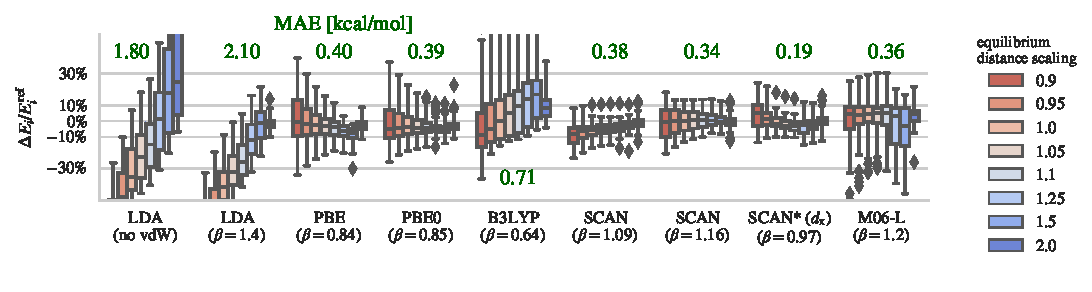
\includegraphics{media/s66-dists}}
\caption{\textbf{Distributions of relative errors in binding energies on the S66x8 set of several DFT+MBD combinations.}
The distributions are displayed as box-and-whisker plots: a box shows the quartiles and whiskers represent the rest of the distribution, except for outliers that are more than 2.5-fold the interquartile distance from the box, which are shown individually.
The $x$-axis labels denote the functional and the value of the MBD range-separation parameter, $\beta^\text{MBD}$.
The blue--red spectrum encodes the scaling, $q$, of the respective equilibrium distances of individual complexes.
The green numbers indicate the mean absolute error (kcal/mol) for $q=1$.
The values of $\beta^\text{MBD}$ were selected as follows: $\beta$-values shown for PBE, PBE0, B3LYP, SCAN* (see text), and M06-L optimize MARE for $q=0.95$--1.05; $\beta=1.4$ for LDA optimizes MARE for $q=2$; and for SCAN and all $q$, $\beta=1.09$ optimizes SDRE, and $\beta=1.16$ optimizes MRE\@.
}\label{fig:s66-dists}
\end{figure*}

\paragraph{VdW benchmark sets from dimers to crystals}

Whereas the vdW models have an explicit correlation range, the range of semilocal density functionals is only implicit, and the combined DFT+vdW models are therefore constructed by optimizing the range separation in vdW models against some benchmark properties, usually binding or lattice energies.
Several benchmark sets of vdW-bound systems have been established, of which we use predominantly three: the S66x8 set of 66 smaller organic dimers~\cite{RezacJCTC11}, the X23 set of 23 molecular crystals~\cite{Otero-de-la-RozaJCP12,ReillyJCP13}, and the S12L set of 12 large supramolecular complexes~\cite{GrimmeCEJ12}.
The S66x8 set is especially useful here, because each of the 66 dimers is given at 8 intermolecular distances distributed around the equilibrium distance, enabling at least partial separation of the short- and long-range behavior of a method.
Further vdW benchmark sets include the 3B-69 set of 3-body interaction energies of small molecules~\cite{RezacJCTC15} and the X40 set of binding energies of halogenated dimers~\cite{RezacJCTC12}.

Here, we shortly discuss only the expected accuracy of the reference values in the benchmark sets, and refer the reader to the cited works for additional details.
The S66x8 set was benchmarked with the coupled-cluster method with single, double, and perturbative triple excitations at the complete basis-set limit (CCSD(T)/CBS), a method that has been itself benchmarked to give at least an order-of-magnitude more accurate binding energies than any of the DFT+vdW methods investigated here~\cite{RezacJCTC13}. % chktex 36
The X23 benchmark lattice energies were obtained from experimental sublimation enthalpies by subtracting the zero-point vibration energy, with the estimated uncertainty of 1\,kcal/mol.
This we recently confirmed by CCSD(T) calculations of the benzene crystal (13.4\,kcal/mol compared to the benchmark value of 12.4\,kcal/mol)~\cite{YangS14}. % chktex 36
The S12L reference binding energies were obtained by subtracting calculated solvation and zero-point energies from experimental free energies of association.
Such a procedure has inherent uncertainty of several kcal/mol, which is supported by recent accurate diffusion quantum Monte Carlo calculations of the bucky-ball--catcher complex ($30\pm1$\,kcal/mol compared to the benchmark value of 27.5\,kcal/mol)~\cite{ZenPRB16}.

The performance of approximate DFT+vdW methods is evaluated by comparing calculated binding energies, $E_i$, to the reference values, $E_i^\text{ref}$, yielding a distribution of errors, $\Delta E_i=E_i-E_i^\text{ref}$.
Since the interaction energies in vdW systems span orders of magnitude, we use relative errors, $\Delta_\mathrm rE_i=\Delta E_i/(-E_i^\text{ref})$ (assuming $E_i$ are negative).
The comparison of error distributions between different methods and systems is aided by introducing various statistical measures.
Two popular measures are the mean absolute error (MAE), $\sum_i\lvert\Delta E_i\rvert/N$, and mean absolute relative error (MARE), $\sum_i\lvert\Delta_\mathrm rE_i\rvert/N$, which both individually serve well as a single numerical indicator of performance, but do not provide much insight into the actual error distributions.
Instead, we use the mean relative error (MRE), $\sum_i\Delta_\mathrm rE_i/N$, and the standard deviation of the relative errors (SDRE),
\[ \text{SDRE}=\frac1N\sqrt{\sum_i(\Delta_\mathrm rE_i-\text{MRE})^2} \]
This enables us to study both the systematic error of a method (overall underbinding or overbinding), represented by MRE, as well as the ``statistical'' error (how consistent a method in terms of the range of errors), represented by SDRE\@.

\section{Results}

\begin{figure*}[t!]
\makebox[\textwidth][c]{
\begin{tikzpicture}
\node[below right, anchor=base] at (0.5,-0.5) {\bfseries a};
\node[below right] at (0,0) {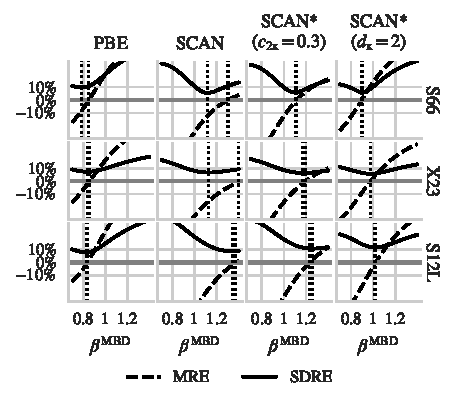
\includegraphics{media/mbd-param-fitting.pdf}};
\node[below right, anchor=base] at (8.1,-0.5) {\bfseries b};
\node[below right] at (7.6,-0.3) {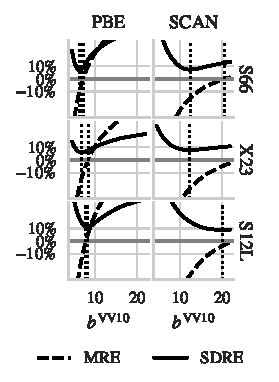
\includegraphics{media/vv10-param-fitting.pdf}};
\node[below right, anchor=base] at (13.6,-0.5) {\bfseries c};
\node[below right] at (13.1,-0.3) {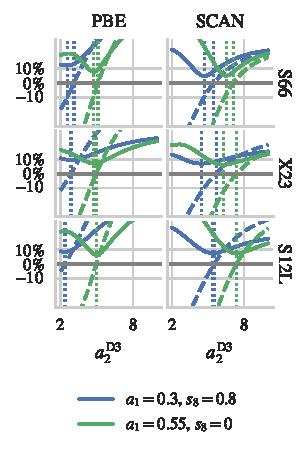
\includegraphics{media/d3-param-fitting.pdf}};
\end{tikzpicture}
}
\caption{\textbf{Dependence of means (MRE) and standard deviations (SDRE) of relative errors in binding energies on range-separation parameters.}
Three long-range correlation models with their respective parameters are shown: (\textbf a) MBD with $\beta^\text{MBD}$, (\textbf b) VV10 with $b^\text{VV10}$, and (\textbf c) D3 with $a_2^\text{D3}$.
Density functionals correspond to columns, and benchmark sets to rows within each subplot.
Only the equilibrium-distance configurations of the S66x8 set are used.
SCAN* denotes two reparameterizations of the SCAN functional discussed in the text. % chktex 36
The vertical dotted lines show where MRE equals to zero or SDRE reaches minimum.
For DFT+D3, two choices are shown of the two other range-separation parameters in D3: $a_1^\text{D3}$ and $s_8^\text{D3}$.
}\label{fig:param-fitting}
\end{figure*}

To study the range of the density functionals LDA, PBE, TPSS, SCAN, PBE0, B3LYP, SCAN0, and M06-L, we evaluated their combinations with the vdW methods MBD, VV10, and D3 at a range of their respective range-separation parameters, on the benchmark sets S66x8, X23, S12L, 3B-69, X40, and on rare-gas dimers.
We analyze the first three (S66x8, X23, S12L) in detail below in Figures~\ref{fig:s66-dists} and~\ref{fig:param-fitting}, whereas the results from 3B-69 (Figure~S1), X40 (Figure~S2) and rare-gas dimers (Figure~S3) are presented in the Supplementary Information because they do not reveal any additional trends in the data.
The full data, obtained with FHI-aims~\cite{BlumCPC09} and Quantum Espresso~\cite{GiannozziJPCM09,HamannPRB13}, as well as computational details and other resources, are published via a Git repository~\cite{GitRepo} and summarized in Supplementary Information.

The case of the S66x8 set and different DFT+MBD combinations (Figure~\ref{fig:s66-dists}) shows that summarizing the error distributions into a single number such as the mean absolute error reduces the method comparison to a one-dimensional classification, whereas comparing the full distributions in fact reveals distinct patterns specific to individual functionals.
Of the tested functionals, LDA is the only one that systematically overbinds S66x8 at equilibrium even without any long-range correction.
At the same time, when the equilibrium distances are scaled by 2, LDA predicts essentially no binding.
In this regard, although LDA binds vdW systems in equilibrium (too) strongly, it is very short-ranged.
The tail behavior can be fixed accurately by MBD with $\beta^\text{MBD}=1.4$, but the short-range overbinding cannot be compensated by a vdW energy term.
The increased overestimation of the XC energy with decreased distance then leads to the well-known underestimation of binding distances by LDA\@.
Already LDA thus illustrates that the degree to which a (semi-)local functional binds vdW systems is in general not a good measure for how well-suited it is for a generally applicable DFT+vdW method. % chktex 36

In contrast, both PBE and PBE0 are strongly underbinding S66x8 at all intermolecular separations, but with MBD and appropriate range separation ($\beta^\text{MBD}\approx0.83$), the resulting PBE+MBD and PBE0+MBD methods are well balanced, with symmetric error distributions, MAE independent of distance, and SDRE monotonously increasing at shorter distances.
The admixture of exact exchange decreases SDRE from 10.2\% with PBE to 8.7\% with PBE0 at equilibrium, but in general has only a small effect.
Another hybrid GGA, B3LYP, behaves as a true opposite of LDA, being at the same time very repulsive, yet quite long-ranged.
Even with a fairly short-range correlation covered by MBD ($\beta^\text{MBD}\approx0.7$), B3LYP+MBD still underbinds at equilibrium, and perhaps more surprisingly at longer distances.
In contrast to PBE/PBE0, the distributions are highly asymmetric, with underbound outliers being mostly the hydrogen-bonded complexes.

With SCAN, optimizing for MRE and SDRE leads to somewhat different values of $\beta^\text{MBD}$, 1.09 and 1.16, respectively, and correspondingly different error distribution profiles.
Both of these $\beta$ values are substantially larger than that for PBE, demonstrating the potentially longer range of SCAN\@.
When SDRE is optimized, SCAN+MBD has consistently narrower error distributions compared to PBE+MBD across all distances, with a slight systematic overbinding that grows with decreasing distances.
When MRE is optimized, the profile of SCAN+MBD is similar to that of PBE+MBD, with smaller outliers.
Adding exact exchange in SCAN0 (not shown) has even smaller effect than in PBE0, making the SCAN and SCAN0 error distributions almost indistinguishable.

Finally, M06-L requires only slightly larger amount of long-range correlation than SCAN, and most of the complexes from the S66x8 set are described well around equilibrium.
But several outliers are strongly overbound, and all complexes are overbound at longer distances, which is in line with previous studies~\cite{GoerigkJPCL15}.
Both issues may stem from the fact that the heavily fitted M06-L is parametrized also on the S22 set, a smaller version of S66x8, but S66x8 contains additional complexes and out-of-equilibrium complexes for which M06-L was not ``trained''.

\begin{table*}[t]
\centering
\caption{\textbf{Overall performance of DFT+MBD/VV10/D3 methods.}}\label{tab:statistics}
\begin{tabular}{lrrrrrrr}
\toprule
XC & \multicolumn3c{MARE$^\text{a}$} & \multicolumn3c{MRE$^\text{b}$} & $^\text{c}$ \\
& S66 & X23 & S12L & S66 & X23 & S12L & \\
\midrule
& \multicolumn6c{MBD} & $\beta^\text{MBD}$ \\
\midrule
    LDA & 32\%  & 21\%  & 12\%  & $-31$\%  & $-17$\%  & 0.1\%    & $\infty$ \\
  B3LYP & 15\%  & 8.0\% & 12\%  & 5.2\%    & $-2.4$\% & 2.5\%    & 0.64     \\
    PBE & 8.4\% & 6.1\% & 5.3\% & $-2.1$\% & $-2.6$\% & $-0.4$\% & 0.84     \\
   PBE0 & 7.6\% & 5.4\% & 6.5\% & $-1.1$\% & $-1.7$\% & $-4.4$\% & 0.85     \\
   SCAN & 4.8\% & 8.4\% & 11\%  & $-3.0$\% & $-7.7$\% & $-10$\%  & 1.12     \\
  M06-L & 9.2\% & 16\%  & 29\%  & 2.4\%    & $-16$\%  & $-28$\%  & 1.20     \\
\midrule
& \multicolumn6c{VV10} & $b^\text{VV10}$ \\
\midrule
    LDA & 36\%  & 37\% & 21\% & $-27\%$  & $-37\%$  & $-21\%$  & $\infty$ \\
  B3LYP & 11\%  & 32\% & 45\% & $-9.3\%$ & $-32\%$  & $-45\%$  & 4.6      \\
    PBE & 9.9\% & 15\% & 15\% & $-6.1\%$ & $-15\%$  & $-15\%$  & 6.8      \\
   PBE0 & 8.3\% & 15\% & 20\% & $-5.3\%$ & $-15\%$  & $-20\%$  & 6.9      \\
   SCAN & 9.3\% & 10\% & 11\% & 2.4\%    & $-9.4\%$ & $-9.9\%$ & 13.7     \\
  M06-L & 11\%  & 17\% & 27\% & 5.5\%    & $-17\%$  & $-27\%$  & 16.2     \\
\midrule
& \multicolumn6c{D3} & $a_2^\text{D3}$ \\
\midrule
    LDA & 33.1\% & 24.9\% & 11.5\% & $-32.2\%$ & $-22.6\%$ & $-2.7\%$  & $\infty$ \\
  B3LYP & 17.0\% & 10.3\% & 16.9\% & 5.4\%     & 2.6\%     & 13.0\%    & 1.62     \\
    PBE & 10.6\% & 7.1\%  & 11.7\% & $-1.1\%$  & 2.7\%     & 10.3\%    & 3.0      \\
   PBE0 & 9.9\%  & 6.2\%  & 9.1\%  & $-1.2\%$  & 3.2\%     & 5.1\%     & 3.1      \\
   SCAN & 6.0\%  & 7.4\%  & 7.1\%  & $-3.8\%$  & $-5.0\%$  & $-5.0\%$  & 5.1      \\
  M06-L & 8.3\%  & 14.5\% & 24.1\% & 0.9\%     & $-14.2\%$ & $-23.5\%$ & 5.6      \\
\bottomrule
\end{tabular}

\small
$^\text{a}$Mean absolute relative error.
$^\text{b}$Mean relative error.
$^\text{c}$Range-separation parameter minimizing MARE on S66x8\@.
\end{table*}

Of the tested functionals, PBE and SCAN (or their hybrid versions) show a potential to work as general balanced DFT+vdW methods.
To rule out the possibility that this conclusion about the two functionals is specific to MBD, we studied how MRE and SDRE of their combinations with MBD, VV10, and D3 depend on the respective range-separation parameters (Figure~\ref{fig:param-fitting}).
Comparing the results for the S66x8 set shows that all three vdW models have similar behavior, including the increased ambiguity in optimizing either for SDRE or MRE on the X23 set in the case of SCAN\@.
It is the case even for D3, which is potentially more flexible when adapting to a functional thanks to its three parameters.
Furthermore, Figure~\ref{fig:param-fitting} shows that whereas the optimal range separation of the vdW models is shared across different system types for the PBE functional, this is not the case for SCAN, for which the XC range seems to grow with the system size (see Figure~S4 for system-size dependence of the binding-energy errors within each dataset).
All these observations are true for all three vdW models.
The results for other functionals are presented in Figure~S5 and summarized in Table~\ref{tab:statistics}.

\begin{figure}[t!]
\makebox[\linewidth][c]{
\begin{tikzpicture}
\node[below right] at (1.1,.1) {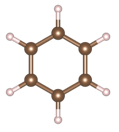
\includegraphics[height=1.2cm]{media/bz2.png}};
\node[below right] at (2.2,.1) {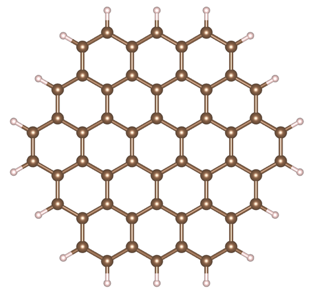
\includegraphics[height=1.2cm]{media/cor21.png}};
\node[below right] at (3.5,.1) {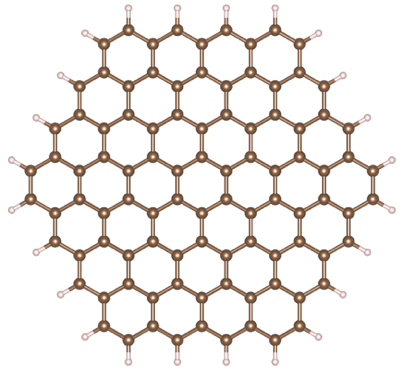
\includegraphics[height=1.2cm]{media/cor22.png}};
\node[below right] at (6.7,0) {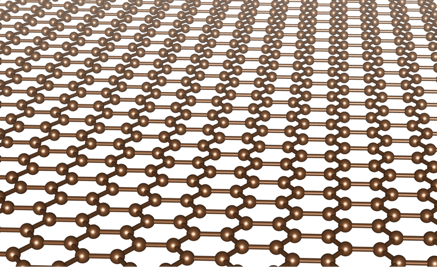
\includegraphics[height=1.0cm]{media/gr2.png}};
\node[below right] at (0,-1) {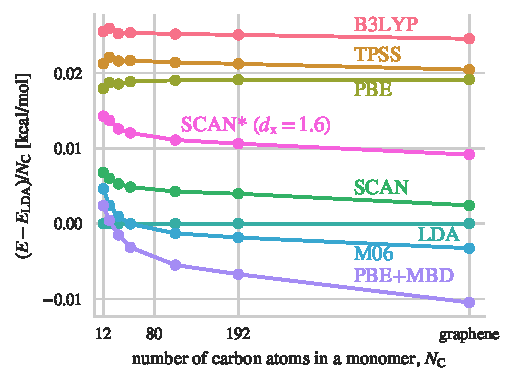
\includegraphics{media/flakes.pdf}};
\end{tikzpicture}
}
\caption{\textbf{Binding energies of graphene-flake dimers.}
The individual data points correspond to (increasing in size) benzene, naphtalene, pyrene, coronene, two larger circular hexagonal flakes (shown), and graphene.
All dimers are in a parallel-displaced configuration, as cut out from a graphite crystal without any geometry relaxations.
The geometries and computational details are available in Supplementary Information.
The plotted quantity is binding energy with respect to the LDA binding energy, per carbon atom.
The (infinite) number of atoms in graphene is set arbitrarily to 500.
}\label{fig:flakes}
\end{figure}

To gain further insight into the range of the functionals beyond statistical analysis, we calculated the binding energies of a series of graphene-flake dimers dimers ranging from a benzene dimer to a graphene bilayer using DFT without any long-range correction (Figure~\ref{fig:flakes}).
We consider LDA as a reference short-range functional, accounting for any potential edge effects, and PBE+MBD as a reference full-range method.
The functionals B3LYP, PBE, and TPSS have a similar behavior to LDA, with the binding energies being offset only by a constant.
In contrast, the SCAN and M06-L show a much stronger dependence on the system size, both at the small and large ends of the spectrum.
The difference in the offset to LDA between benzene dimer and graphene is 60\% for M06-L and 35\% for SCAN with respect to PBE+MBD\@.
The ability to capture at least partially this system-size effect could be seen as advantageous, but it is unfortunate for developing DFT+vdW methods, because it breaks the core assumption that the functionals behave as short-range models of the electron correlation.
After all, these functionals are semilocal by construction and the fact that they are sensitive to this strongly nonlocal environment is contradicting this semilocality.
Furthermore, there are no known nontrivial exact constraints on the XC energy of overlapping density tails, and so the behavior of current semilocal functionals for such systems is essentially an uncontrolled result of the overall functional design, which complicates any development of ``farsighted'' density functionals.
The fact that a semilocal functional can capture a nonlocal information about the system in the first place (besides that contained implicitly in the electron density) can be understood by recognizing that the kinetic energy density, while being an explicit local function, is in fact an implicit nonlocal functional of the electron density.

Both SCAN and M06-L are meta-GGAs, but so is TPSS, which does not show this sensitivity.
We speculate that in the case of SCAN, this sensitivity is caused by the particular parametrization of its dependence on the dimensionless electron localization parameter, $\alpha$ (see Background).
The values of $\alpha$ typically count in single figures within the electronic valence shells and decay close to zero with distance from the electronic system, while crossing $\alpha=1$ at some point~\cite{SunPRL13,BeckeJCP90}.
(This is followed either by asymptotic decay to zero in the case of valence $s$-like orbitals, or asymptotic increase to infinity in all other cases.)
Among meta-GGA functionals, SCAN has a relatively wide plateau around $\alpha=1$ (due to Eq.~\ref{eq:scan-interp})~\cite{LoosJCP17}, where the interpolating function is equal to 1, and the functional dependence of $F_\text X$ becomes that of the fourth order expansion around the uniform electron gas.
This results in spatial regions in the electron density tails (dominated by HOMO, the highest-occupied molecular orbital) that are described with a uniform-like functional instead of the more appropriate single-orbital form of $\alpha\approx0$.
This can lead to sudden spikes in the exchange-correlation potential fairly outside the spatial regions where covalent bonding occurs~\cite{Gerit-private}.

\begin{figure}[t!]
\centering
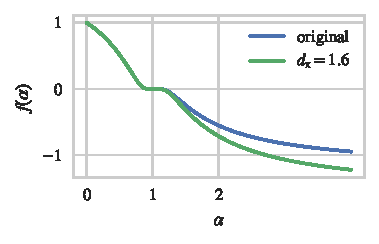
\includegraphics{media/scan-interp}
\caption{\textbf{Interpolation and extrapolation used in the SCAN exchange functional.}
The fixed points that are inter- and extrapolated are $\alpha=0$ and $\alpha=1$.
The shape of the function is controlled with three parameters, $c_\mathrm{1x}=0.667$, $c_\mathrm{2x}=0.8$, and $d_\mathrm x=1.24$ (original values).
}\label{fig:scan-interp}
\end{figure}

In the series of graphene-flake dimers, the electronic gap (calculated with SCAN) decreases from 4.7\,eV for benzene dimer to 0.9\,eV for graphene bilayer, which makes the density tail decay slower with increasing system size.
Because the $\alpha=1$ behavior of SCAN makes it quite sensitive in the density tails, whose overlap also encodes the vdW bonding on the electron-density level, it only makes sense that SCAN is able to extract the nonlocal information about the system size via the decreasing electronic gap.
This mechanism could be also partially responsible for the discrepancies in optimal range separation for SCAN observed on the S66x8, X23, and S12L sets (Figure~\ref{fig:param-fitting}).

To check this hypothesis, we constructed several reparameterizations of SCAN and tested them on these benchmark sets.
We focused on the three parameters in Eq.~\ref{eq:scan-interp} because their values are determined weakly, having been fitted only to system-specific rather than universal norms.
We found that the overall XC range of SCAN can be changed substantially by modifying either of these parameters, without any regression in the overall performance of the SCAN+vdW methods.
However, the systems-size dependence of the optimal range separation for SCAN is not affected by either of them.
For illustration, Figures~\ref{fig:s66-dists},~\ref{fig:param-fitting}, and~\ref{fig:flakes} show results for a SCAN reparametrization with $d_\mathrm x$ changed from 1.24 to 1.6, which minimizes the overall error on S66x8 and reduces the XC range of SCAN (optimal $\beta^\text{MBD}$ of 0.97).
Figure~\ref{fig:flakes} clearly shows that the reparameterization does not change the sensitivity of SCAN in the density tails, as it only shifts the binding energy in graphene flakes by a constant.

\section{Discussion}

SCAN has been previously combined with VV10 by \citet{PengPRX16} and with D3 and VV10 by \citet{BrandenburgPRB16}.
The obtained optimal values of $b^\text{VV10}$ were 15.7 and 14.0, respectively, and optimal parametrization of D3 was found to be $s_8^\text{D3}=0$, $a_1^\text{D3}=0.54$ and $a_2^\text{D3}=5.4$.
From the results in Figure~\ref{fig:param-fitting}, this corresponds to an optimal MRE on S66x8 for SCAN+VV10 (but systematic overbinding on X23 and S12L), and to optimal statistical error (SDRE) for SCAN+D3, leading again to some degree of systematic overbinding.
\citet{BrandenburgPRB16} associated this tendency mainly with hydrogen-bonded systems, which is in line with the observed overbinding of various ice structures by SCAN (without any vdW correction)~\cite{ChenPRB16}.

\citet{PengPRX16} argued that shifting the range separation between a semilocal functional and a vdW model towards the latter is beneficial.
Such a shift could also avoid some of the problems that long-range correlation models need to deal with at short range, such as the quadrupole interaction.
Our results confirm that such a shift is indeed possible in principle, but with the caveat that the description of the intermediate range by the density functional must be balanced and independent of system size.

Our toy reparameterization of the SCAN functional illustrates that the XC range of even a very sophisticated functional can be changed by a single parameter, whose value is not fixed by any physical constraint.
At the same time, it shows that a more subtle behavior of the XC range such as the system-size dependence is likely a result of the inherent functional form rather than a specific value of a numerical parameter.
Furthermore, we did not evaluate any other properties besides vdW binding, and it is quite possible that the new parameter values would introduce regressions for other systems.
To give a true alternative parametrization, the original fitting procedure would need to be performed with an additional constraint on vdW binding, perhaps expressed via a single simple system, which is beyond the scope of this work.

The results on the graphene flakes, which do not use any vdW method, as well as those on the vdW benchmark sets, which are universal across three different vdW methods, suggest that modifying the SCAN functional would be a more straightforward approach to fixing the observed issues with the range separation.
That being said, it is certainly possible in principle to attack the problem from the other side, and try to develop a more complex range-separation scheme in the different vdW models, which would fit the effective range of the SCAN (or another meta-GGA) functional.
However, such a scheme would certainly require explicit consideration of the functional form of meta-GGA functionals, and perhaps incorporation of the dependence on the density parameter $\alpha$.

\section{Conclusions}

We showed that although the range of semilocal functionals cannot be known explicitly, it is still possible to obtain meaningful and detailed information about their range by probing them with long-range correlation models, for which the range is known explicitly.
This information can be then used to construct the functionals in such a way that their range is consistent across different systems, a condition necessary for a generally applicable DFT+vdW method.
After all, semilocal functionals and vdW methods model two interconnected parts of the electron correlation, and it is reasonable to develop them in tandem.
